% ------------------------------------------------------------------------------
% TYPO3 v9 LTS - What's New (English Version)
%
% @author	Michael Schams <schams.net>
% @license	Creative Commons BY-NC-SA 3.0
% @link		https://typo3.org/help/documentation/whats-new/
% @language	English
% ------------------------------------------------------------------------------

\section{Introduction}
\begin{frame}[fragile]
	\frametitle{Introduction}

	\begin{center}\huge{\color{typo3darkgrey}\textbf{Introduction}}\end{center}
	\begin{center}\large{\textit{Key facts and figures}}\end{center}

\end{frame}

% ------------------------------------------------------------------------------
% TYPO3 CMS 9 LTS - The Facts

\begin{frame}[fragile]
	\frametitle{Introduction}
	\framesubtitle{TYPO3 v9 LTS}

	\begin{itemize}
		\item Release date: 2 October 2018
		\item Release type: LTS release (Long Term Release)
		\item Development time: 18 months
	\end{itemize}

	\begin{figure}
		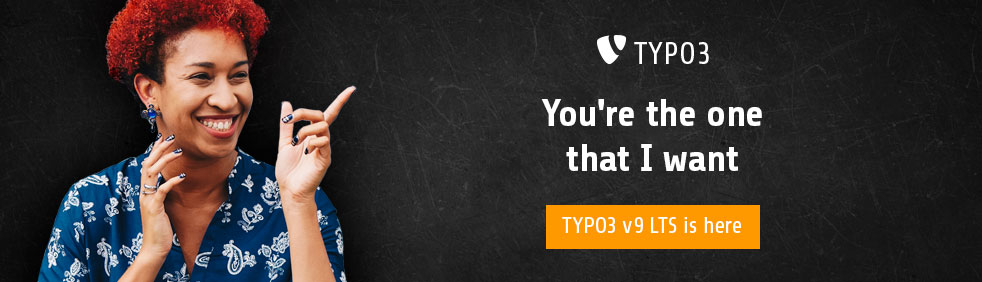
\includegraphics[width=0.95\linewidth]{Introduction/typo3-v95-banner.jpg}
	\end{figure}

\end{frame}

% ------------------------------------------------------------------------------
% System Requirements

\begin{frame}[fragile]
	\frametitle{Introduction}
	\framesubtitle{System Requirements}

	\begin{itemize}
		\item PHP version 7.2+
		\item Required PHP settings:

			\begin{itemize}
				\item \texttt{memory\_limit} >= 256M
				\item \texttt{max\_execution\_time} >= 240s
				\item \texttt{max\_input\_vars} >= 1500
				\item compilation option \texttt{-}\texttt{-disable-ipv6} must \underline{not} be used
			\end{itemize}

		\item Required PHP extensions:\newline
			\small
				filter, hash, openssl, pcre >= 8.38, session, SPL, standard,
				xml, zip and zlib
			\normalsize
	\end{itemize}

\end{frame}

% ------------------------------------------------------------------------------
% System Requirements

\begin{frame}[fragile]
	\frametitle{Introduction}
	\framesubtitle{System Requirements}

	\begin{itemize}
		\item Webserver such as Apache, Nginx, IIS, etc.
		\item All databases supported by \textbf{Doctrine DBAL} are also
			supported by TYPO3. For example:
	\end{itemize}

	\begin{figure}
		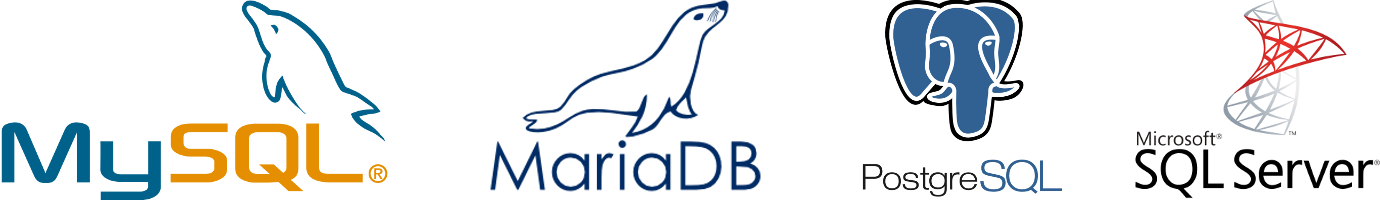
\includegraphics[width=0.70\linewidth]{Introduction/logo-databases.png}
	\end{figure}

	\begin{itemize}
		\item Minimum disk space required: 200 MB
		\item The backend requires Microsoft Internet Explorer 11 or later,
			Microsoft Edge, Google Chrome, Firefox, Safari or any other modern,
			compatible browser
	\end{itemize}

\end{frame}

% ------------------------------------------------------------------------------
% Sprint Releases

\begin{frame}[fragile]
	\frametitle{Introduction}
	\framesubtitle{Development Timeline}

	Sprint Releases published:

	\begin{itemize}
		\item v9.0 \tabto{1.1cm}12/Dec/2017\tabto{3.4cm}Install Tool and Page Tree Refactoring,\newline
			\tabto{3.4cm}Unified Page Translations
		\item v9.1 \tabto{1.1cm}30/Jan/2018\tabto{3.4cm}Redirect Handling
		\item v9.2 \tabto{1.1cm}10/Apr/2018\tabto{3.4cm}Site Handling
		\item v9.3 \tabto{1.1cm}12/Jun/2018\tabto{3.4cm}SEO and URL Routing Preparations
		\item v9.4 \tabto{1.1cm}04/Sep/2018\tabto{3.4cm}URL Routing for Pages
		\item v9.5 \tabto{1.1cm}02/Oct/2018\tabto{3.4cm}LTS Preparation and Release
	\end{itemize}

\end{frame}

% ------------------------------------------------------------------------------
% LTS Support Timeline

\begin{frame}[fragile]
	\frametitle{Introduction}
	\framesubtitle{Long Term Support}

	\begin{figure}
		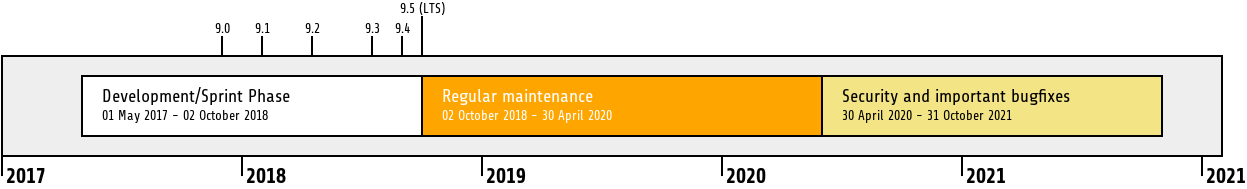
\includegraphics[width=1\linewidth]{Introduction/typo3-v9-lifecycle.png}
	\end{figure}

	\begin{itemize}
		\item TYPO3 version 9.5 is a LTS release (Long Term Support)
		\item Regular maintenance and bugfixes until March 2020
		\item Security and critical bugfixes until October 2021
	\end{itemize}
	\vspace{0.2cm}
	\textbf{Extended Support}\newline
	\smaller
		\href{https://typo3.com}{TYPO3 GmbH} offers Extended Long Term
			Support (ELTS) for TYPO3 v9 LTS until October 2024.
	\normalsize

\end{frame}

% ------------------------------------------------------------------------------
